\subsection{About ktlint}
Ktlint is a popular an anti-bikeshedding Kotlin linter with a built-in formatter created by pinterest. It tries to reflect official code style from \texttt{kotlinlang.org} and Android Kotlin Style Guide and then automatically apply these rules to your codebase. Ktlint can check and automatically fix code. IIt claims to be simple and easy to use. As it is focused more on checking code-style and code-smell related issues, ktlint inspections are working with Abstract Syntax Tree generated by Kotlin parser. Ktlint framework has some basic utilities to make the work with Kotlin AST easier, but anyway all inspections work with original ASTNode provided by Kotlin parser.

Ktlint has been developed since 2016 and from then on it has 3.8k stars, 309 forks and 390 closed PRs (2020). It looks to be the most popular and mature linter in the Kotlin community right now. There have been written ~15k lines of code.

Ktlint has it’s own set of rules, which are divided on standard and experimental rules. But unfortunately the number of fixers and checkers in the standard ruleset is very few (~20 rules) and inspections are trivial. 

Ktlint can be used as a plugin for Maven, Gradle or command line app. To configure rules in Ktlint you should modify \texttt{.editorconfig} file - this is the only configuration that ktlint provides and it contains just simple configuration like the number of spaces in indents. Actually you even can’t configure specific rules (for example to disable or suppress any of them), instead you can provide some common settings like the number of spaces for indenting. In other words, ktlint has a "fixed hardcoded” code-style that is not very configurable. 

If you want to implement your own rules you need to create a your own Ruleset. Ktlint is very user-friendly for creation of custom Rulesets. In this case ktlint will parse the code using a Kotlin parser and will trigger your inspection (as visitor) for each and every node of AST. Ktlint is using java’s \texttt{ServiceLoader} to discover all available Rulesets. \texttt{ServiceLoader} is used to inject your own implementation of rules for the static analysis. In this case ktlint becomes a third-party dependency and a framework. Basically you should provide implementation of \texttt{RuleSetProvider} interface.

Ktlint refers to article on medium on how to create a custom Ruleset and a Rule.

A lot of projects uses ktlint as their code formatting tool. For example, OmiseGo \footnote{\url{https://github.com/omgnetwork/android-sdk}} (currently rebranding to OMG Network) - a quite popular cryptocurrency.

To summarize: Ktlint is very mature and useful as a framework for creating your own checker\&fixer of Kotlin code and doing AST-analysis. It can be very useful if you need only simple inspections that check (and fix) code-style issues (like indents).

\begin{figure}[H]
    \centering
    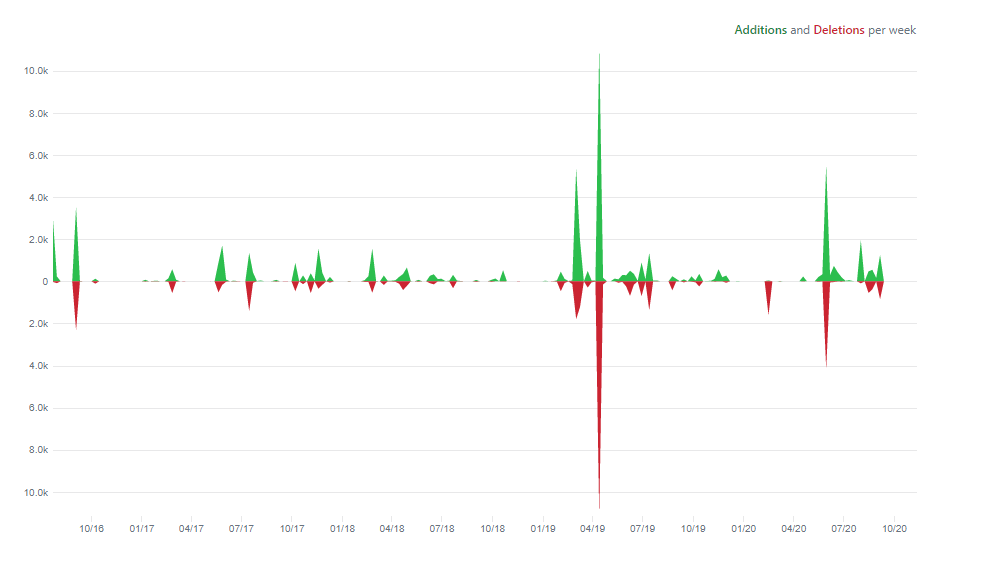
\includegraphics[scale = 0.3]{pictures/ktlint.png}
    \caption{Ktlint Code Frequency}
    \label{fig:png_ktlint}
\end{figure}

\subsection{About detekt}
Detekt \footnote{\url{https://github.com/detekt/detekt}} is a static code analysis tool. It operates on an abstract syntax tree (AST) and meta-information provided by Kotlin compiler. On the top of that info, it does a complex analysis of the code. However, this project is more focused on checking the code rather than fixing. Similarly, to ktlint, it has it’s own rules and inspections. Detekt uses wrapped ktlint to redefine RuleSet of ktlint as it’s formatting rules.

Detekt supports detection of code smells, bugs searching and code-style checking. It has a highly configurable rule sets (can even make suppression of issues from the code). And the number of checkers is quite big: it has more than 100 inspections. Detekt has IntelliJ integration, third-party integrations for Maven, Bazel and Github actions and a mechanism for suppression of their warnings with @Suppress annotation from the code. It is being developed since 2016 and today it has 3.2k stars, 411 forks and 1850 closed PRs. It has about 45k lines of code. And it’s codebase is the biggest comparing to other analyzers.
Detekt is used in such projects as fountain \footnote{\url{https://github.com/xmartlabs/fountain}} or Kaspresso   \footnote{\url{https://github.com/KasperskyLab/Kaspresso}}.

To summarize: Detekt is very useful as a Kotlin static analyser for CI/CD. It tries to find bugs in the code and is focused more on checking of the code. Detekt has 100+ rules that check the code.

\begin{figure}[H]
    \centering
    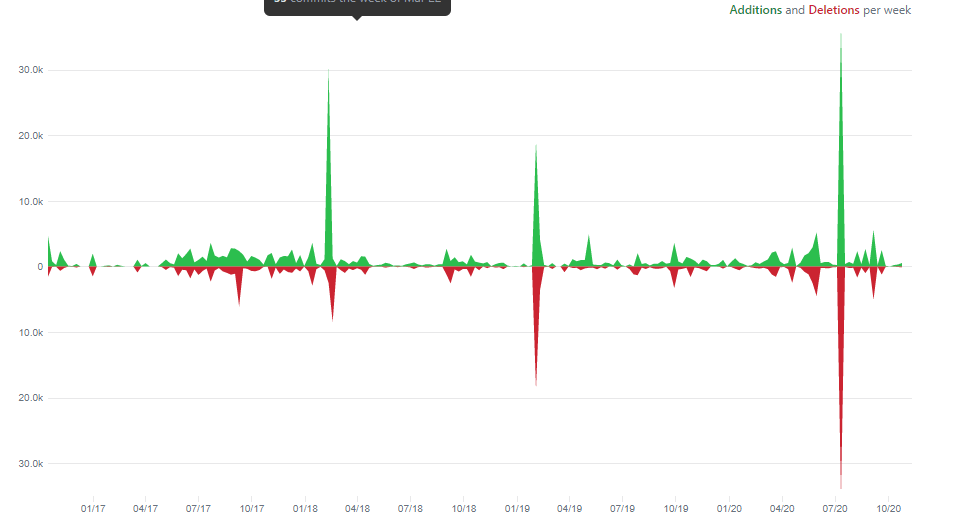
\includegraphics[scale = 0.3]{pictures/detekt.png}
    \caption{Detekt Code Frequency}
    \label{fig:png_detekt}
\end{figure}

\subsection{About ktfmt}
Ktfmt is a program that formats Kotlin code, based on google-java-format. It's development has started in Facebook in the end of 2019. It can be added to your project through a Maven dependency, Gradle dependency, IntelliJ plugin or you can run it through a command line. Ktfmt is not a configurable application, so to change any rule logic you need to download the project and redefine some constants. Ktfmt has 214 stars, 16 forks, 20 closed PRs and around 7500 lines of code. 

To summarize: no one knows why Facebook has invested their money in this tool. Nothing new was not introduced. If they really needed to have new rules - they could have created their own Ruleset for ktlint or detekt.

\begin{figure}[H]
    \centering
    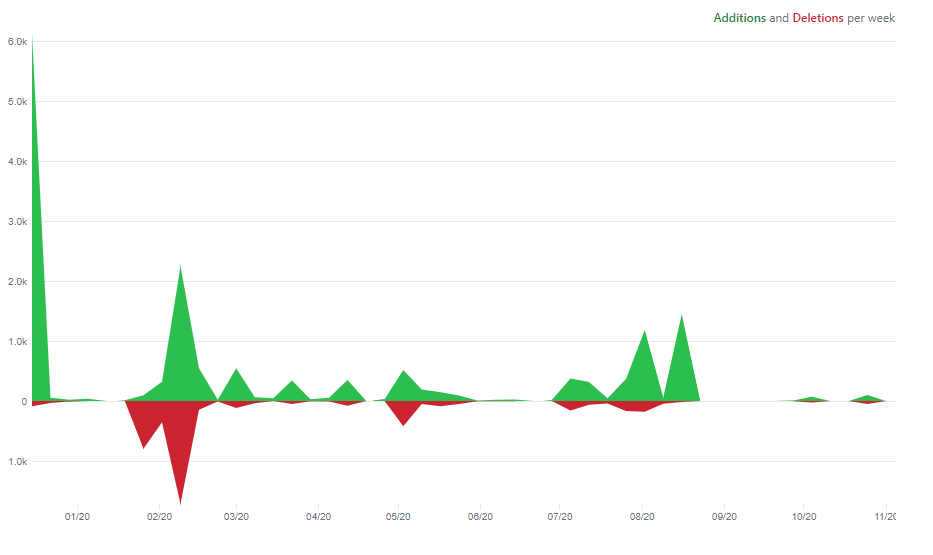
\includegraphics[scale = 0.3]{pictures/ktfmt.png}
    \caption{Ktfmt Code Frequency}
    \label{fig:png_ktfmt}
\end{figure}

\subsection{About diKTat}
Diktat as well as ktlint and detekt is a static code analysis tool. But diktat is not only a tool, but also a coding convention that in details describes all the rules that you should follow when writing a code on Kotlin. It’s development has started in 2020 and at the time of writing this article diKTat has 168 stars and 13 forks. DiKTat operates on AST provided by kotlin compiler. So why diKTat is better?

First of all, it supports much more rules than ktlint. It’s ruleset includes more than 100 rules, that can both check and fix your code.

Second, diKTat is configurable. A lot of rules have their own settings, and all of them can be easily understood. For example, you can choose whether you need a copyright, choose a length of line or you can configure your indents.

Third, diKTat is very easy to configure. You don’t need to spend hours only to understand what each rule is doing. Diktat’s ruleset is a \texttt{.yml} file, where each rule is commented out with the description. Also you can suppress error on the particular lines of code using \texttt{@Suppress} annotation in your code.

DiKTat can be used as a CI/CD tool in order to avoid merging errors in the code. Overall it can find code smells and code style issues. Also it can find pretty not obvious bugs by complex AST analysis. Diktat works with maven, gradle and as command-line application powered by ktlint.

To summarize: diktat contains a strict coding convention that was not yet introduced by other linters. It works both as a checker and as a fixer. Diktat has much more inspections (100+) and is very configurable (each inspection can be disabled/configured separately), so you can configure it for your particular project.

\begin{figure}[H]
    \centering
    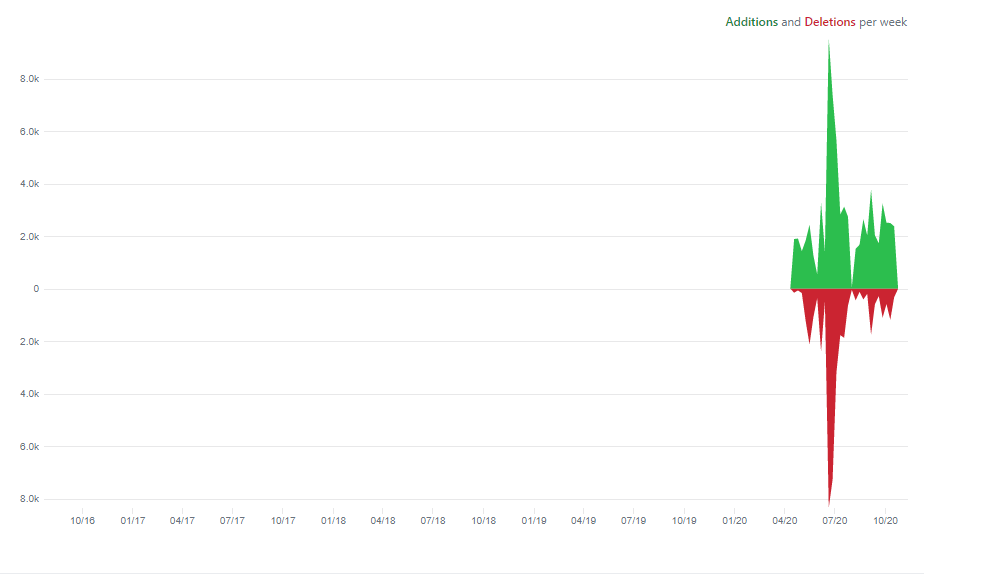
\includegraphics[scale = 0.3]{pictures/diktat.png}
    \caption{DiKTat Code Frequency}
    \label{fig:png_diktat}
\end{figure}

\subsection{A few words about Jetbrains}
Jetbrains invented  Kotlin and created one of the best IDEs for Java and Kotlin called IntelliJ. This IDE supports a built-in linter. However, it is not a well-configurable tool, you are not able to specify your own coding convention and it is not useful for CI/CD as it is highly coupled with UI. Unfortunately such static analysis is not so effective as it cannot prevent merging of the code with bugs into the repository. As experience shows - many developers simply ignore those static analysis errors until they are blocked from merging their pull requests. So it is not so suitable for CI/CD, but very good for finding and fixing issues inside your IDE.

\subsection{Summary}

\begin{center}
\begin{tabular}{ |p{3cm}|p{2.5cm}|p{2.5cm}|p{2.5cm}|p{2.5cm}| }
\hline
\multicolumn{5}{|c|}{\textbf{Comparing table}} \\
\hline
& diKTat& ktlint &detekt & ktfmt \\
\hline
starting year & 2020 & 2016 & 2016 & 2019 \\
stars & 168 & 3.2k & 3.8k & 214\\ 
forks & 13 & 299 & 411 & 16\\
closed PRs & 321 & 390 & 1850 & 20 \\
lines of code & 32k & 15k & 45k & 7,5k\\
number of rules & $>$100 & $\approx$ 20 & $>$100 & $\approx$ 10 \\
is configurable & yes & no & yes/no & no \\
maven/gradle plugin & both & both & gradle only & no \\
web version & yes & yes & no & no \\
\hline

\hline
\end{tabular}
\end{center}